\documentclass[11pt,a4paper]{article}

% ---------------------------------------------------------------- packages
\usepackage[margin=1in]{geometry}
\usepackage[T1]{fontenc}
\usepackage{lmodern}
\usepackage{microtype}
\usepackage{amsmath,amssymb}
\usepackage{booktabs}
\usepackage{tabularx}
\usepackage{array}
\usepackage{graphicx}
\usepackage[table]{xcolor}
\usepackage{tikz}
\usetikzlibrary{arrows.meta,positioning}
\usepackage{pgfplots}
\pgfplotsset{compat=1.18}
\usepackage{algorithm}
\usepackage{algpseudocode}
\usepackage{enumitem}
\usepackage[section]{placeins}
\usepackage[font=small,labelfont=bf]{caption}
\usepackage[numbers,sort&compress]{natbib}
\usepackage[hidelinks]{hyperref}

\definecolor{smlindigo}{HTML}{4F46E5}
\definecolor{smlcyan}{HTML}{06B6D4}
\definecolor{smlslate}{HTML}{94A3B8}
\definecolor{smlamber}{HTML}{F59E0B}
\definecolor{smlnavy}{HTML}{0B1224}

\newcommand{\sys}{SML}
\newcommand{\best}[1]{\textbf{#1}}
\newcolumntype{Y}{>{\raggedright\arraybackslash}X}
\setlist{itemsep=2pt,topsep=4pt}

\title{\textbf{Governed Shared Memory for Cross-Team AI Agents:\\
Permission-Aware Hybrid Retrieval with Versioning and Auditability}}

\author{
  {[Student Name]}\thanks{Replace the bracketed placeholders with the author details before submission.}\\
  \small Department of Computer Science and Engineering, {[Institute Name]}\\
  \small \texttt{{[student-email]}}
  \and
  {[Guide Name]}\\
  \small Department of Computer Science and Engineering, {[Institute Name]}\\
  \small \texttt{{[guide-email]}}
}
\date{September 2026}

\begin{document}
\maketitle

% ================================================================ abstract
\begin{abstract}
Large-language-model (LLM) agents are increasingly deployed per team---for development, quality assurance,
security and customer support---but each agent keeps a private memory. The result is repeated
investigation, duplicated reasoning cost, knowledge silos and contradictory records. Pooling all agent
knowledge into a single vector database is not an acceptable fix, because semantic similarity is not
authorisation: a support agent's question can retrieve a confidential security finding. We present the
\emph{Shared Memory Layer} (\sys{}), a service through which agents of different teams store, retrieve,
share and version knowledge under explicit governance. \sys{} expresses one access-control predicate in
three enforcement forms---application code, SQL and a vector-store filter---so that unauthorised memories are
never scored by the similarity search and every candidate is re-checked against the system of record. It
combines dense and full-text retrieval under the same filter, keeps immutable versions and provenance,
flags duplicates and contradictions for human review, and writes an append-only audit trail. Agents
connect through a REST API, the Model Context Protocol and client SDKs. On an in-house cross-team benchmark,
sharing raised Hit@1 from 0.35 to 0.975 and removed all duplicated work (62.5\,\% $\rightarrow$ 0\,\%), while 0 of
140 adversarial access attempts leaked. On three public benchmarks the permission-aware hybrid search
outperformed BM25 and a plain vector store: Recall@10 of 0.673 on LoCoMo (the benchmark authors' DRAGON
retriever: 0.675), 0.807 on LongMemEval and nDCG@10 of 0.718 / 0.359 on BEIR SciFact / NFCorpus, with a
33M-parameter local embedding model and a median search latency of 83--109\,ms at up to 102{,}229 memories.
\end{abstract}

\noindent\textbf{Keywords:} multi-agent systems; agent memory; retrieval-augmented generation; access
control; vector search; hybrid retrieval; auditability.

% ================================================================ 1 introduction
\section{Introduction}

AI agents now write code, test releases, review security findings and answer customers. In most
deployments each agent is configured per team and keeps its own memory, whether that memory is a chat
history, a scratch-pad file or a private vector index. When the Development agent learns that
authentication fails because refresh tokens expire, the QA agent that meets the same symptom a week later
cannot benefit: it re-investigates, spends the same LLM reasoning budget again, and may record a slightly
different---or contradictory---conclusion. The organisation pays repeatedly for knowledge it already has.

The obvious remedy, one shared vector database, introduces a security problem that is easy to miss.
Semantic search ranks every stored item by similarity to the query. If confidential memories are part of
the index, a harmless-looking question from an unauthorised agent can retrieve them, and any filter applied
\emph{after} ranking is a single point of failure. Organisations also need what a plain index does not
offer: who created a piece of knowledge, how it changed, whether two agents disagree, and who read or was
refused access.

This paper describes and evaluates the Shared Memory Layer (\sys{}), a governed memory service for agents
of different teams. Its central idea is that authorisation must be part of retrieval, not a step after it.
Our contributions are:
\begin{enumerate}[leftmargin=*]
  \item \textbf{A single access predicate in three enforcement forms.} One read rule over five visibility
  levels is implemented as application logic, as a SQL predicate and as a vector-store payload filter.
  Similarity search therefore never scores an unreadable memory, and every result is re-checked against
  the relational system of record (Section~\ref{sec:access}).
  \item \textbf{Permission-aware hybrid retrieval.} Dense nearest-neighbour search and PostgreSQL full-text
  search run under the identical filter and are merged with a transparent scoring function
  (Section~\ref{sec:retrieval}).
  \item \textbf{Knowledge governance.} Immutable versions, provenance, semantic duplicate detection,
  rule-based contradiction flags with human review, and an append-only audit log that records denials
  (Section~\ref{sec:lifecycle}).
  \item \textbf{A complete, open implementation} with REST, Model Context Protocol (MCP) and SDK interfaces,
  a dashboard and one-command deployment (Section~\ref{sec:impl}).
  \item \textbf{An evaluation} on an in-house cross-team benchmark, an adversarial security suite and three
  public benchmarks---LoCoMo, LongMemEval and BEIR---against BM25, a plain vector store and published
  results of other memory layers (Section~\ref{sec:eval}).
\end{enumerate}

% ================================================================ 2 related work
\section{Related Work}
\label{sec:related}

\paragraph{Multi-agent LLM frameworks.} AutoGen~\cite{wu2023autogen}, MetaGPT~\cite{hong2024metagpt} and
CAMEL~\cite{li2023camel} coordinate several LLM agents through conversation or a shared message pool.
Shared state lives for one run or one group chat; there is no persistent, access-controlled memory across
teams. Conceptually \sys{} is a governed \emph{blackboard}~\cite{wooldridge2009mas}: agents coordinate
indirectly through persistent knowledge instead of point-to-point messages.

\paragraph{Memory for LLM agents.} Generative Agents~\cite{park2023generative} retrieve from a memory
stream by recency, importance and relevance; MemGPT~\cite{packer2023memgpt} pages information between a
context window and external storage. Production memory layers such as Mem0~\cite{chhikara2025mem0},
Zep~\cite{rasmussen2025zep}, LangMem~\cite{langmem2025} and A-Mem~\cite{xu2025amem} extract facts or build
(temporal) knowledge graphs with an LLM at ingestion time and report answer accuracy on long-conversation
benchmarks. These systems optimise memory for one user or one agent; scoping is by user, agent or project
identifier. None of the published evaluations addresses per-memory authorisation across teams, leakage
under similarity attacks or auditability, which are the focus of this work.

\paragraph{Retrieval.} Retrieval-augmented generation~\cite{lewis2020rag} conditions an LLM on retrieved
text. Dense retrievers~\cite{reimers2019sbert,karpukhin2020dpr,lin2023dragon} and general-purpose embedding
models such as BGE~\cite{xiao2023cpack} and MiniLM~\cite{wang2020minilm} capture meaning beyond shared
words; lexical ranking with BM25~\cite{robertson2009bm25} remains a strong baseline for exact terms, and
late-interaction models such as ColBERT~\cite{khattab2020colbert} trade cost for quality. BEIR~\cite{thakur2021beir}
and MTEB~\cite{muennighoff2023mteb} are the standard benchmarks for these components. Approximate nearest
neighbour search with HNSW graphs~\cite{malkov2020hnsw} underlies vector databases such as
Qdrant~\cite{qdrant2024}, which can evaluate payload filters inside the index.

\paragraph{Access control.} Role-based access control (RBAC)~\cite{sandhu1996rbac} governs \emph{operations};
attribute-based access control (ABAC)~\cite{hu2014abac} evaluates attributes of subjects and objects.
\sys{} combines RBAC for operations with attribute-based, per-object visibility for memories.

Table~\ref{tab:related} summarises the gap.

\begin{table}[htbp]
\centering
\small
\caption{Capabilities of related approaches ($\checkmark$ supported, $\sim$ partial / session-scoped / via
extensions, -- not addressed), assessed from the designs described in the cited papers and documentation.}
\label{tab:related}
\begin{tabularx}{\textwidth}{@{}>{\raggedright\arraybackslash}p{4.3cm}*{6}{>{\centering\arraybackslash}X}@{}}
\toprule
Approach & Persistent memory & Cross-team sharing & Semantic retrieval & Per-memory access control & Versions \& provenance & Security audit trail \\
\midrule
AutoGen, MetaGPT, CAMEL & $\sim$ & $\sim$ & $\sim$ & -- & -- & -- \\
Generative Agents, MemGPT & $\checkmark$ & -- & $\checkmark$ & -- & -- & -- \\
RAG over a vector store & $\checkmark$ & $\sim$ & $\checkmark$ & $\sim$ & -- & -- \\
Mem0 & $\checkmark$ & $\sim$ & $\checkmark$ & $\sim$ & $\sim$ & -- \\
Zep & $\checkmark$ & $\sim$ & $\checkmark$ & -- & $\sim$ & -- \\
\midrule
\textbf{\sys{} (this work)} & $\checkmark$ & $\checkmark$ & $\checkmark$ & $\checkmark$ & $\checkmark$ & $\checkmark$ \\
\bottomrule
\end{tabularx}
\end{table}

% ================================================================ 3 problem
\section{Problem Formulation and Threat Model}
\label{sec:problem}

\paragraph{Entities.} An organisation has teams $\mathcal{T}$. A \emph{principal} $p$ is either an agent
(with its own API key) or a human user; it belongs to at most one team $\tau(p)$, holds one or more roles
and thereby a set of permissions (e.g.\ \texttt{memory:create}, \texttt{memory:read},
\texttt{memory:share}). A \emph{memory} $m$ has a title, content, type, tags, importance and confidence
in $[0,1]$, an owning team $\tau(m)$, a creator $c(m)$, a visibility $v(m)$, a sensitivity level
(public, internal, confidential, restricted), an optional expiry time, explicit sharing grants to teams
$G_T(m)$ and agents $G_A(m)$, and a version history.

\paragraph{Visibility.} Table~\ref{tab:visibility} lists the five visibility levels. Confidential and
restricted memories may not be organisation-wide.

\begin{table}[htbp]
\centering
\small
\caption{Memory visibility levels.}
\label{tab:visibility}
\begin{tabular}{@{}ll@{}}
\toprule
Visibility & Readable by (besides the creator and administrators) \\
\midrule
\texttt{private} & nobody else; private memories cannot be shared \\
\texttt{team} & members of the owning team, plus explicit team or agent grants \\
\texttt{selected\_teams} & the owning team plus the explicitly allowed teams \\
\texttt{selected\_agents} & only the explicitly allowed agents \\
\texttt{organization} & every authenticated principal \\
\bottomrule
\end{tabular}
\end{table}

\paragraph{Read predicate.} For a non-administrator principal $p$ holding \texttt{memory:read}, memory
$m$ is readable, $R(p,m)$, if and only if $m$ is active, not expired (unless expired memories are
explicitly requested), and
\begin{equation}
\begin{split}
& c(m) = p \;\lor\; v(m) = \texttt{organization} \\
& \lor\; \Big( v(m) \neq \texttt{private} \;\land\; \big[ \big(\tau(p) = \tau(m) \land v(m) \in \{\texttt{team}, \texttt{selected\_teams}\}\big) \\
& \qquad\qquad \lor\; \tau(p) \in G_T(m) \;\lor\; p \in G_A(m) \big] \Big).
\end{split}
\label{eq:read}
\end{equation}
Archived memories are visible to administrators only. Modification (update, archive, share) additionally
requires the creator or a manager of the owning team.

\paragraph{Goals.} (G1) An agent can retrieve, by meaning, every memory it is authorised to read,
including other teams' knowledge. (G2) No operation---read, search, update, version history,
sharing---discloses a memory for which $R(p,m)$ is false, including through similarity ranking,
duplicate warnings or conflict notices. (G3) Every change is versioned and attributable. (G4) Every access
and every refusal is recorded in a tamper-resistant log.

\paragraph{Adversary.} We consider authenticated but unauthorised principals: agents of other teams who
issue arbitrary requests, including semantic searches that use the protected memory's own title or
content as the query (the strongest similarity attack), attempts to share a memory to themselves, and
privilege escalation (creating teams or agents, reading the audit log, listing users, re-indexing). Token
theft is mitigated by short-lived tokens and refresh-token rotation; compromise of the database or of the
host is out of scope.

% ================================================================ 4 design
\section{System Design}
\label{sec:design}

\subsection{Architecture}

Figure~\ref{fig:arch} shows the components. Agents and human users call a single API gateway. Every
request is authenticated (a JWT~\cite{rfc7519} or an agent API key) and authorised twice: RBAC decides
whether the principal may perform the operation, and the read predicate~\eqref{eq:read} decides whether it
may touch the specific memory. PostgreSQL is the system of record for memories, versions, grants,
identities and the audit log. Qdrant stores one vector per memory together with the payload fields needed to
evaluate the read predicate. Embeddings are produced locally by \texttt{bge-small-en-v1.5}~\cite{xiao2023cpack}
(384 dimensions, 33M parameters), so no text leaves the deployment.

\begin{figure}[htbp]
\centering
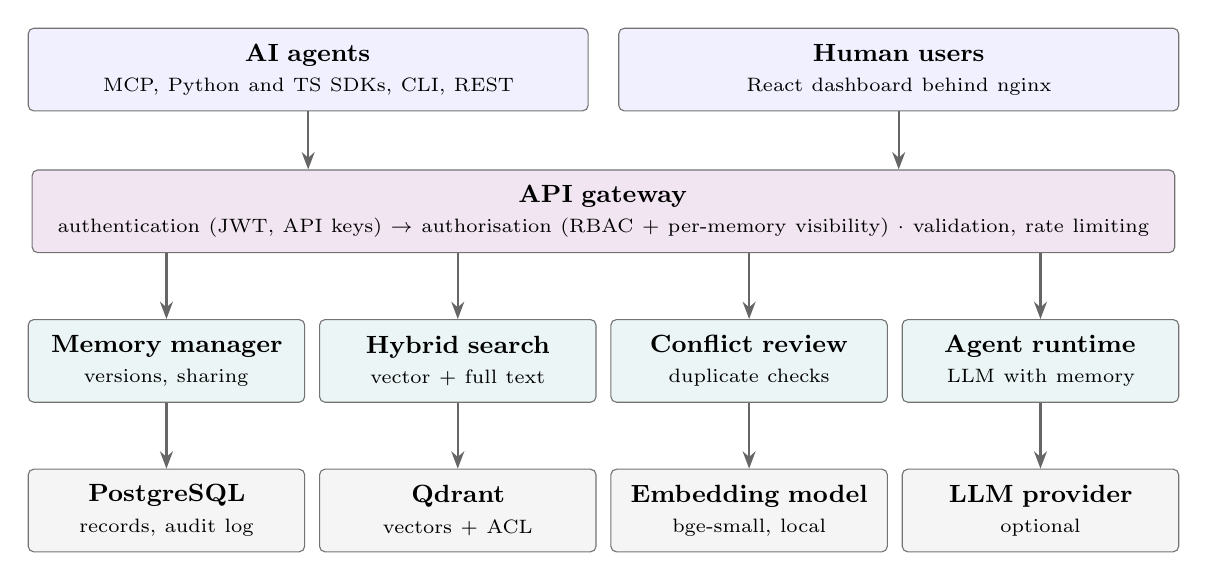
\begin{tikzpicture}[
  box/.style={draw=black!55, rounded corners=2pt, align=center, font=\small, inner sep=3pt, minimum height=1.05cm, fill=#1, execute at begin node={\hyphenpenalty=10000\exhyphenpenalty=10000}},
  box/.default=white,
  arr/.style={-{Stealth[length=2.2mm]}, thick, black!60}]
\node[box=blue!6, text width=6.9cm] (agents) at (-3.75,0) {\textbf{AI agents}\\\scriptsize MCP, Python and TS SDKs, CLI, REST};
\node[box=blue!6, text width=6.9cm] (humans) at (3.75,0) {\textbf{Human users}\\\scriptsize React dashboard behind nginx};
\node[box=violet!10, text width=14.3cm] (gw) at (0,-1.8) {\textbf{API gateway}\\\scriptsize authentication (JWT, API keys) $\rightarrow$ authorisation (RBAC + per-memory visibility) $\cdot$ validation, rate limiting};
\node[box=teal!8, text width=3.3cm] (s1) at (-5.55,-3.7) {\textbf{Memory manager}\\\scriptsize versions, sharing};
\node[box=teal!8, text width=3.3cm] (s2) at (-1.85,-3.7) {\textbf{Hybrid search}\\\scriptsize vector + full text};
\node[box=teal!8, text width=3.3cm] (s3) at (1.85,-3.7) {\textbf{Conflict review}\\\scriptsize duplicate checks};
\node[box=teal!8, text width=3.3cm] (s4) at (5.55,-3.7) {\textbf{Agent runtime}\\\scriptsize LLM with memory};
\node[box=gray!8, text width=3.3cm] (d1) at (-5.55,-5.6) {\textbf{PostgreSQL}\\\scriptsize records, audit log};
\node[box=gray!8, text width=3.3cm] (d2) at (-1.85,-5.6) {\textbf{Qdrant}\\\scriptsize vectors + ACL};
\node[box=gray!8, text width=3.3cm] (d3) at (1.85,-5.6) {\textbf{Embedding model}\\\scriptsize bge-small, local};
\node[box=gray!8, text width=3.3cm] (d4) at (5.55,-5.6) {\textbf{LLM provider}\\\scriptsize optional};
\draw[arr] (agents.south) -- (agents.south |- gw.north);
\draw[arr] (humans.south) -- (humans.south |- gw.north);
\foreach \x in {s1,s2,s3,s4} { \draw[arr] (\x.north |- gw.south) -- (\x.north); }
\draw[arr] (s1.south) -- (d1.north);
\draw[arr] (s2.south) -- (d2.north);
\draw[arr] (s3.south) -- (d3.north);
\draw[arr] (s4.south) -- (d4.north);
\end{tikzpicture}
\caption{Architecture of the Shared Memory Layer. Every path to a memory passes through authentication and
two-level authorisation; audit records are written in an independent transaction.}
\label{fig:arch}
\end{figure}

\subsection{One access rule, three enforcement forms}
\label{sec:access}

A naive design ranks all memories by similarity and filters the results afterwards. Two failure modes
follow: unreadable memories still participate in ranking (and can surface in any code path that forgets the
filter), and a single bug in the post-filter exposes everything. \sys{} instead implements the read predicate
\eqref{eq:read} three times and keeps the forms synchronised by tests:
\begin{enumerate}[leftmargin=*]
  \item \texttt{can\_read} evaluates a concrete PostgreSQL row and is authoritative;
  \item \texttt{sql\_read\_filter} is a SQL predicate used for listings and full-text search;
  \item \texttt{build\_read\_filter} is a Qdrant payload filter (a disjunction of conjunctions over
  visibility, owning team, creator, grants, status and expiry) that is pushed \emph{into} the
  approximate nearest-neighbour query.
\end{enumerate}
Because the filter is part of the vector query, an unreadable memory is never a candidate, however
similar it is. Every candidate is nevertheless re-checked with \texttt{can\_read} against the current row
before it is returned (defence in depth, and protection against a stale vector payload). Duplicate warnings
are computed only among readable memories, and conflicts with unreadable memories are reported to
administrators while the caller only learns their count.

\subsection{Permission-aware hybrid retrieval}
\label{sec:retrieval}

Embeddings capture paraphrase but blur exact identifiers such as error codes, CVE numbers or ticket ids.
\sys{} therefore runs two candidate generators under the same filter (Algorithm~\ref{alg:search}): a dense
search in Qdrant and a PostgreSQL full-text search~\cite{postgres2023fts} over a generated, weighted
\texttt{tsvector} (title weight A, content weight B) with \texttt{websearch\_to\_tsquery}, in which every
query term must match. Keyword-only candidates receive their true cosine similarity from Qdrant, so all
candidates are scored on the same scale:
\begin{equation}
s(m) = 0.90\,\mathrm{sim}(q,m) + 0.05\,\mathrm{imp}(m) + 0.05\,\mathrm{conf}(m) + 0.02\,[\mathrm{verified}(m)] + 0.10\,\mathrm{kw}(q,m),
\label{eq:score}
\end{equation}
where $\mathrm{kw}$ is the \texttt{ts\_rank\_cd} rank normalised by the best keyword hit (0 for memories
that do not contain every query term). The weights favour meaning, let human-verified and high-confidence
knowledge win ties, and give exact matches a bonus. If the vector store is unavailable, search degrades to
permission-filtered keyword search instead of failing.

\begin{algorithm}[htbp]
\caption{Permission-aware hybrid search}
\label{alg:search}
\begin{algorithmic}[1]
\Require principal $p$, query $q$, metadata filters $F$, result size $k$
\State $\phi \gets \textsc{ReadFilter}(p) \land F$ \Comment{visibility, grants, status, expiry, type, project, \dots}
\State $C_{\mathrm{kw}} \gets$ full-text matches of $q$ in PostgreSQL under $\phi$ (all terms), ranked by \texttt{ts\_rank\_cd}
\State $\mathbf{v} \gets \textsc{Embed}(q)$
\State $C_{\mathrm{vec}} \gets$ the $3k$ nearest neighbours of $\mathbf{v}$ in Qdrant under $\phi$
\State $C \gets C_{\mathrm{kw}} \cup C_{\mathrm{vec}}$; obtain cosine similarity for keyword-only candidates
\ForAll{$m \in C$}
  \If{\textbf{not} \textsc{CanRead}$(p, m)$ on the current PostgreSQL row}
    \State remove $m$ from $C$ \Comment{defence in depth}
  \EndIf
  \State compute $s(m)$ with Equation~\eqref{eq:score}
\EndFor
\State update access and cross-team reuse counters; append a \texttt{MEMORY\_SEARCH} audit record
\State \Return the $k$ highest-scoring memories of $C$
\end{algorithmic}
\end{algorithm}

\subsection{Write path, lifecycle and governance}
\label{sec:lifecycle}

\paragraph{Creation.} A new memory is validated (lengths, tag format, no markup in titles, sensitivity
rules), authorised (\texttt{memory:create}; the body may not name another agent or team), embedded, and
checked for duplicates: an identical content hash or a readable memory with cosine similarity
$\geq 0.92$ yields a warning (or a rejection, if requested). Organisation-wide candidates with similarity
$\geq 0.70$ are passed to contradiction rules (e.g.\ differing numeric values or opposite technology
choices for the same subject), which open a conflict for human review. The row, version~1 and grants are
flushed to PostgreSQL, the vector is upserted into Qdrant, and the transaction commits; if the commit
fails the vector is deleted, and an administrator endpoint reports and repairs any divergence by
re-embedding from PostgreSQL.

\paragraph{Versioning and provenance.} Updates lock the row, check an optional expected version
(optimistic concurrency), increment the version and store an immutable snapshot linked to its predecessor.
There is exactly one vector per memory, so search always returns the latest version while older versions
remain readable to authorised principals. Provenance reports the creator, source, modifiers and access
history. Humans resolve conflicts with \emph{keep new}, \emph{keep existing}, \emph{keep both} or
\emph{dismiss}; nothing is silently overwritten.

\paragraph{Auditability.} Logins, token events, every memory operation, sharing changes, role and
permission changes, conflict resolutions and every denial are recorded with actor, team,
\emph{on-behalf-of} principal, resource, status, reason and request identifier. Audit writes use an
independent transaction, so refused operations are always recorded, and a database trigger rejects
\texttt{UPDATE} and \texttt{DELETE} on the audit table.

\paragraph{Identity security.} Passwords are hashed with Argon2id~\cite{biryukov2016argon2}. Access tokens
are HS256 JWTs valid for 15 minutes; opaque refresh tokens rotate on every use, and re-use of a rotated
token revokes its whole family. Agent API keys are stored only as keyed hashes. Authentication endpoints
are rate limited per client and repeated failures lock an account temporarily.

\subsection{Agent interfaces}

\begin{sloppypar}
Agents use \sys{} through (i) a REST API documented with OpenAPI (57 operations), (ii) a Model Context
Protocol~\cite{anthropic2024mcp} endpoint exposing eight tools---\texttt{search\_memory}, \texttt{remember},
\texttt{get\_memory}, \texttt{update\_memory}, \texttt{share\_memory}, \texttt{memory\_history},
\texttt{list\_teams}, \texttt{whoami}---so that off-the-shelf MCP clients can use the memory without code,
and (iii) Python and TypeScript SDKs with a command-line tool, bulk import of Markdown, JSON and CSV
knowledge, and ready-made tool definitions for LLM function calling. All interfaces execute as the calling
agent through the same services, so authorisation, rate limits and auditing are identical. A built-in
agent runtime retrieves memories for a task, passes them to a configurable LLM (local or hosted) and can
store the result as a new memory.
\end{sloppypar}

% ================================================================ 5 implementation
\section{Implementation}
\label{sec:impl}

\sys{} is implemented in Python~3.12 with FastAPI and Pydantic~v2 (API), SQLAlchemy~2 and Alembic
(PostgreSQL~16 schema with foreign keys, check constraints, indexes, a generated full-text column and the
append-only audit trigger), Qdrant~1.13 (HNSW with payload indexes on every filter field) and fastembed/ONNX
for local embeddings. A React/TypeScript dashboard provides monitoring, a memory explorer, access-control
management, the audit log, a conflict-review queue and an \emph{agent playground} in which a human
simulates an agent under that agent's permissions (audited on the human's behalf). The whole system runs
as four containers with one \texttt{docker compose} command. The test suite comprises 105 backend tests
(unit, security and integration tests against real PostgreSQL, Qdrant and the embedding model, including an
end-to-end MCP test with the official client), 14 Python SDK tests, 5 TypeScript SDK tests and a 16-step
acceptance scenario against the running deployment; all pass.

% ================================================================ 6 evaluation
\section{Evaluation}
\label{sec:eval}

We answer four questions. \textbf{RQ1:} does shared memory improve retrieval and reduce duplicated work
compared with per-agent memory? \textbf{RQ2:} does the access model prevent leakage, including through
similarity? \textbf{RQ3:} how good is the retrieval on public benchmarks compared with standard baselines
and published systems? \textbf{RQ4:} what latency does governed retrieval cost?

\subsection{Setup}

All experiments ran on one laptop (Windows~11 on ARM64, Docker Desktop with 12 virtual CPUs and 15.5\,GB of
memory; no GPU). Every memory was created and every question asked through the public API as an ordinary,
permission-checked request. The public benchmarks ran against a second API process from the same image with
its own database and collection (rate limiting disabled on that process only), so the 100{,}000+ benchmark
memories did not affect the demonstration data or its audit log. Two baselines ran locally over exactly the
same texts: \textbf{BM25}~\cite{robertson2009bm25} ($k_1{=}1.5$, $b{=}0.75$) and a \textbf{plain vector store}
using \texttt{all-MiniLM-L6-v2}~\cite{wang2020minilm,reimers2019sbert} with cosine similarity, the default
embedding model of Chroma-style memories. We report \sys{} in \emph{hybrid} (default) and \emph{semantic}
(dense only) mode. Published results of other systems are quoted from their papers and were not re-run.

\paragraph{Validity of the scoring.} Our local \texttt{all-MiniLM-L6-v2} baseline reproduces its published
BEIR scores exactly (nDCG@10 0.645 on SciFact and 0.316 on NFCorpus, as in the MTEB results), and \sys{}'s
semantic mode reproduces the published scores of \texttt{bge-small-en-v1.5} (0.717 vs.\ 0.713 and 0.342 vs.\
0.343). The LongMemEval metrics were ported line by line from the official evaluation code and agree with it
to $10^{-16}$ on 3{,}000 randomised rankings. Retrieval is deterministic: two independent LoCoMo runs
produced identical recall.

\subsection{RQ1: Shared versus isolated memory}

\paragraph{Corpus.} Four freshly created team agents (Development, QA, Security, Support) stored 35 labelled
memories; 40 paraphrased questions (10 per team) have ground-truth relevant memories, and 25 of them can only
be answered with another team's knowledge. \emph{Isolated} restricts each agent to its own memories (the
per-agent silo), \emph{Shared} is \sys{}, and \emph{Lexical} ranks exactly the memories the agent may read
with TF-IDF, separating the effect of embeddings from the effect of sharing.

\begin{table}[htbp]
\centering
\small
\caption{In-house cross-team benchmark (35 memories, 40 queries, top-5).}
\label{tab:inhouse}
\begin{tabular}{@{}lccc@{}}
\toprule
Metric & Isolated (baseline) & \textbf{Shared (\sys{})} & Lexical (TF-IDF) \\
\midrule
Hit@1 & 0.350 & \best{0.975} & 0.850 \\
Hit@5 & 0.375 & \best{1.000} & \best{1.000} \\
Recall@5 & 0.338 & 0.963 & \best{0.988} \\
MRR & 0.358 & \best{0.983} & 0.921 \\
nDCG@5 & 0.338 & \best{0.957} & 0.927 \\
Hit@5 on the 25 cross-team queries & 0.000 & \best{1.000} & \best{1.000} \\
Knowledge-reuse rate & 0.000 & \best{0.675} & -- \\
\midrule
Tasks resolved from existing memory & 0.375 & \best{1.000} & -- \\
Duplicate-task rate (knowledge re-derived) & 0.625 & \best{0.000} & -- \\
Re-derived memories flagged as duplicates & 25 / 25 & -- & -- \\
\bottomrule
\end{tabular}
\end{table}

Table~\ref{tab:inhouse} shows that sharing is what makes the cross-team questions answerable at all (Hit@5
0.375 $\rightarrow$ 1.000), while embeddings mainly improve \emph{ranking} over keyword matching on the same
authorised memories (Hit@1 0.850 $\rightarrow$ 0.975). In agent tasks, isolated agents had to re-derive
62.5\,\% of the answers; every one of those 25 re-stored memories was flagged by \sys{}'s duplicate
detector. Without an LLM the shared agent completed tasks in 122\,ms on average versus 265\,ms for the
isolated agent including re-derivation. With a small local LLM (\texttt{qwen2.5:0.5b} on CPU) the shared agent
was about 20\,\% slower (4{,}283 vs.\ 3{,}574\,ms) because it sends more retrieved context to the model, but
every answer was grounded in existing organisational knowledge.

\subsection{RQ2: Security}

The adversarial suite let every agent outside the authorised teams attack each of seven protected memories
through six paths, plus five privilege-escalation operations (Table~\ref{tab:security}).

\begin{table}[htbp]
\centering
\small
\caption{Adversarial security suite.}
\label{tab:security}
\begin{tabularx}{0.85\textwidth}{@{}Ycc@{}}
\toprule
Attempt & Attempts & Blocked \\
\midrule
Direct read of a protected memory & 20 & 20 \\
Update & 20 & 20 \\
Read version history & 20 & 20 \\
Share the memory to one's own team & 20 & 20 \\
Semantic search using the memory's title & 20 & 20 \\
Semantic search using the memory's full content & 20 & 20 \\
Privilege escalation (create team / agent, read audit log, list users, re-index) & 20 & 20 \\
\midrule
\textbf{Total} & \textbf{140} & \textbf{140} \\
\bottomrule
\end{tabularx}
\end{table}

No attempt leaked, including the 40 searches that used the protected memory's own text as the query; the
protected memories were never scored. All 100 expected denials were found in the audit log (the 40 search
attempts are not denials and are audited as ordinary searches).

\subsection{RQ3: Public benchmarks}

\begin{figure}[htbp]
\centering
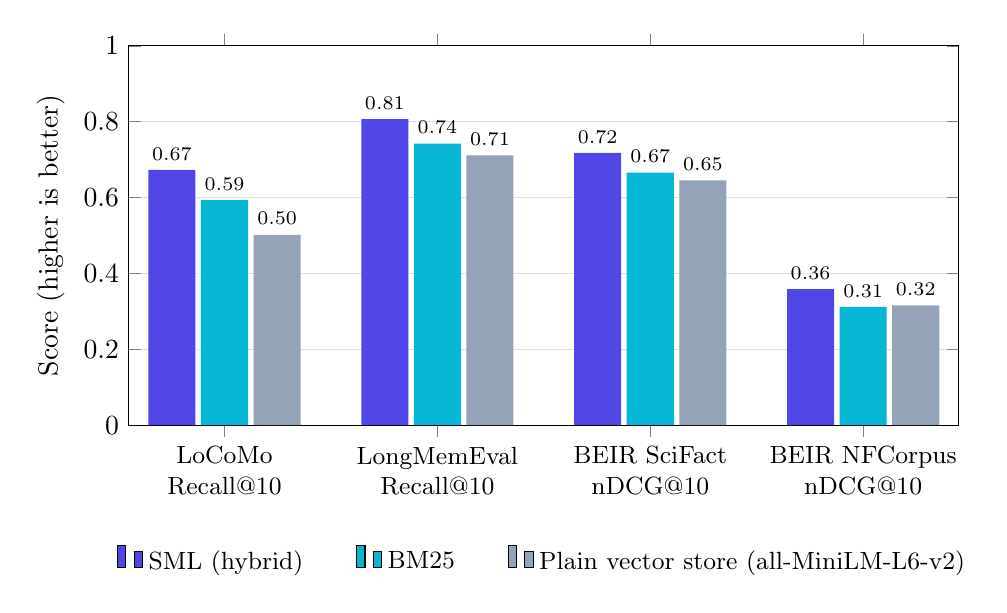
\begin{tikzpicture}
\begin{axis}[
  ybar,
  bar width=17pt,
  width=\textwidth,
  height=6.4cm,
  ymin=0, ymax=1.0,
  ylabel={Score (higher is better)},
  symbolic x coords={LoCoMo,LongMemEval,SciFact,NFCorpus},
  xtick=data,
  xticklabels={{LoCoMo\\Recall@10},{LongMemEval\\Recall@10},{BEIR SciFact\\nDCG@10},{BEIR NFCorpus\\nDCG@10}},
  xticklabel style={align=center, font=\small},
  enlarge x limits=0.15,
  ymajorgrids=true,
  grid style={gray!25},
  nodes near coords={\pgfmathprintnumber[fixed zerofill,precision=2]{\pgfplotspointmeta}},
  every node near coord/.append style={font=\scriptsize},
  legend style={at={(0.5,-0.3)}, anchor=north, legend columns=-1, draw=none, font=\small, /tikz/every even column/.append style={column sep=0.6cm}},
  legend cell align=left,
]
\addplot[fill=smlindigo, draw=none] coordinates {(LoCoMo,0.673) (LongMemEval,0.807) (SciFact,0.718) (NFCorpus,0.359)};
\addplot[fill=smlcyan, draw=none] coordinates {(LoCoMo,0.593) (LongMemEval,0.742) (SciFact,0.666) (NFCorpus,0.312)};
\addplot[fill=smlslate, draw=none] coordinates {(LoCoMo,0.502) (LongMemEval,0.711) (SciFact,0.645) (NFCorpus,0.316)};
\legend{\sys{} (hybrid), BM25, Plain vector store (all-MiniLM-L6-v2)}
\end{axis}
\end{tikzpicture}
\caption{Headline metric of each public benchmark for \sys{} and the two baselines run on identical data.}
\label{fig:overview}
\end{figure}

Figure~\ref{fig:overview} summarises the headline metric of each benchmark; details follow.

\paragraph{LoCoMo.} LoCoMo~\cite{maharana2024locomo} contains very long multi-session conversations with
questions whose evidence turns are annotated; it is the benchmark on which Mem0, Zep, LangMem and A-Mem report.
We stored all 5{,}882 turns of the 10 released conversations (one project per conversation) and evaluated the
1{,}535 answerable questions (the adversarial category is excluded, as in the Mem0 evaluation). Recall@$k$ is
the share of evidence turns retrieved in the top $k$, the metric the LoCoMo authors report for their DRAGON
retriever~\cite{lin2023dragon}.

\begin{table}[htbp]
\centering
\small
\caption{LoCoMo evidence retrieval (1{,}535 questions). Bold: best measured value per column.}
\label{tab:locomo}
\begin{tabular}{@{}lccccccc@{}}
\toprule
Configuration & R@5 & R@10 & R@25 & R@50 & Hit@1 & MRR & nDCG@10 \\
\midrule
\sys{} hybrid & \best{0.582} & \best{0.673} & \best{0.789} & \best{0.852} & \best{0.392} & \best{0.511} & \best{0.523} \\
\sys{} semantic & 0.561 & 0.657 & 0.783 & 0.848 & 0.352 & 0.478 & 0.494 \\
\sys{} keyword only (all terms) & 0.119 & 0.121 & 0.122 & 0.123 & 0.118 & 0.126 & 0.118 \\
BM25 & 0.523 & 0.593 & 0.669 & 0.719 & 0.345 & 0.450 & 0.463 \\
Plain vector store & 0.397 & 0.502 & 0.637 & 0.729 & 0.212 & 0.326 & 0.344 \\
Recency (last $k$ turns) & 0.002 & 0.010 & 0.034 & 0.078 & 0.001 & 0.005 & 0.004 \\
\midrule
\textit{DRAGON (published, 50 conv.)} & \textit{0.588} & \textit{0.675} & \textit{0.799} & \textit{0.848} & -- & -- & -- \\
\bottomrule
\end{tabular}
\end{table}

\begin{figure}[htbp]
\centering
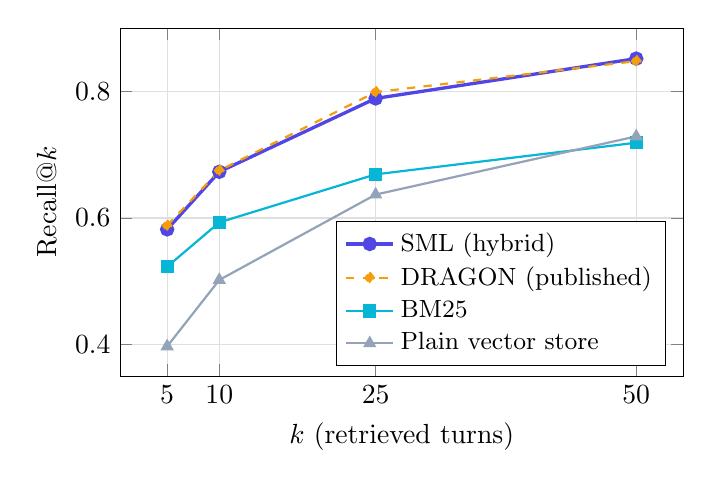
\begin{tikzpicture}
\begin{axis}[
  width=0.72\textwidth,
  height=6cm,
  xlabel={$k$ (retrieved turns)},
  ylabel={Recall@$k$},
  xtick={5,10,25,50},
  ymin=0.35, ymax=0.9,
  grid=major,
  grid style={gray!25},
  legend pos=south east,
  legend style={font=\small},
  legend cell align=left,
]
\addplot[smlindigo, very thick, mark=*] coordinates {(5,0.582) (10,0.673) (25,0.789) (50,0.852)};
\addplot[smlamber, thick, dashed, mark=diamond*] coordinates {(5,0.588) (10,0.675) (25,0.799) (50,0.848)};
\addplot[smlcyan, thick, mark=square*] coordinates {(5,0.523) (10,0.593) (25,0.669) (50,0.719)};
\addplot[smlslate, thick, mark=triangle*] coordinates {(5,0.397) (10,0.502) (25,0.637) (50,0.729)};
\legend{\sys{} (hybrid), DRAGON (published), BM25, Plain vector store}
\end{axis}
\end{tikzpicture}
\caption{LoCoMo Recall@$k$: \sys{} is within 0.01 of the benchmark authors' DRAGON retriever at every depth.}
\label{fig:locomo}
\end{figure}

\begin{table}[htbp]
\centering
\small
\caption{LoCoMo Recall@10 by question category (number of questions).}
\label{tab:locomocat}
\begin{tabular}{@{}lcccc@{}}
\toprule
Configuration & Single-hop (841) & Temporal (320) & Multi-hop (282) & Open-domain (92) \\
\midrule
\sys{} hybrid & \best{0.733} & \best{0.736} & \best{0.488} & \best{0.473} \\
\sys{} semantic & 0.711 & 0.720 & 0.485 & \best{0.473} \\
BM25 & 0.699 & 0.688 & 0.277 & 0.267 \\
Plain vector store & 0.570 & 0.562 & 0.309 & 0.266 \\
\bottomrule
\end{tabular}
\end{table}

Hybrid retrieval is the best configuration at every cut-off (Table~\ref{tab:locomo}) and tracks DRAGON within
0.01 (Figure~\ref{fig:locomo}), although DRAGON has roughly three times as many parameters and was evaluated
on the full 50-conversation set; we therefore read the result as \emph{comparable}, not better. The margin
over BM25 is largest on multi-hop and open-domain questions (+0.21 Recall@10, Table~\ref{tab:locomocat}), which
paraphrase their evidence. Requiring every query term (keyword-only mode) is precise but recalls evidence for
only 12\,\% of questions, which is why \sys{} uses full-text search as a bonus rather than as the primary
ranker. The top-10 context is about 441 tokens, 2\,\% of an average conversation (about 21{,}475 tokens).

\paragraph{LongMemEval.} LongMemEval~\cite{wu2025longmemeval} evaluates the long-term memory of chat
assistants: each question has its own history of about 48 sessions (about 115k tokens). We used
LongMemEval$_S$ and followed the official retrieval protocol: every user message is a retrievable item,
evidence messages are annotated, abstention questions and questions whose evidence lies only in assistant
messages are skipped, Recall@$k$ requires \emph{all} evidence messages in the top $k$, and session-level
metrics are derived from the message ranking. This yields 419 questions; storing each question's history in
its own project produced 102{,}229 memories.

\begin{table}[htbp]
\centering
\small
\caption{LongMemEval$_S$ retrieval (419 questions, official protocol). The published Stella~V5 1.5B
results~\cite{wu2025longmemeval,stella2024} use LongMemEval$_M$, whose haystack is about ten times larger,
and are a reference point only.}
\label{tab:lme}
\begin{tabular}{@{}lcccccc@{}}
\toprule
 & \multicolumn{5}{c}{Message level} & Session level \\
\cmidrule(lr){2-6}\cmidrule(l){7-7}
Configuration & R@5 & NDCG@5 & R@10 & NDCG@10 & R@50 & R@10 \\
\midrule
\sys{} hybrid & \best{0.637} & 0.663 & \best{0.807} & \best{0.708} & \best{0.974} & 0.907 \\
\sys{} semantic & \best{0.637} & 0.656 & 0.802 & 0.700 & \best{0.974} & \best{0.909} \\
BM25 & 0.628 & \best{0.664} & 0.742 & 0.693 & 0.840 & 0.783 \\
Plain vector store & 0.511 & 0.570 & 0.711 & 0.623 & 0.936 & 0.840 \\
\midrule
\textit{Stella V5 1.5B on $M$ (published)} & \textit{0.582} & \textit{0.481} & \textit{0.692} & \textit{0.512} & -- & \textit{0.783} \\
\bottomrule
\end{tabular}
\end{table}

\begin{table}[htbp]
\centering
\small
\caption{LongMemEval$_S$ message-level Recall@10 by question type (number of questions).}
\label{tab:lmetype}
\begin{tabular}{@{}lcccccc@{}}
\toprule
Configuration & Multi-session & Temporal & Knowl.\ update & User facts & Preferences & Assistant \\
 & (121) & (127) & (72) & (64) & (30) & (5) \\
\midrule
\sys{} hybrid & \best{0.711} & 0.732 & \best{0.958} & 0.953 & \best{0.800} & \best{1.000} \\
\sys{} semantic & \best{0.711} & 0.724 & \best{0.958} & 0.938 & \best{0.800} & \best{1.000} \\
BM25 & 0.562 & \best{0.748} & 0.931 & \best{0.969} & 0.500 & 0.800 \\
Plain vector store & 0.545 & 0.614 & 0.903 & 0.953 & 0.767 & \best{1.000} \\
\bottomrule
\end{tabular}
\end{table}

\sys{} retrieves all evidence within the top 10 for 80.7\,\% of the questions and within the top 50 for
97.4\,\% (Table~\ref{tab:lme}); at least one evidence message is in the top 10 for 93.8\,\%. The largest
gains over BM25 are on multi-session and preference questions (Table~\ref{tab:lmetype}), whose wording differs
from the evidence. BM25 is marginally ahead on temporal and user-fact questions, which repeat exact names and
dates, and ties \sys{} on NDCG@5. Because the full-text component rewards only memories containing every query
term, it rarely fires on long natural-language questions; a BM25-weighted lexical ranking fused with the
dense ranking (e.g.\ reciprocal rank fusion~\cite{cormack2009rrf}) is the natural next step.

\paragraph{BEIR.} BEIR~\cite{thakur2021beir} measures zero-shot document retrieval, the component every
memory layer depends on. We ingested SciFact (5{,}183 abstracts, 300 claims) and NFCorpus (3{,}633 medical
documents, 323 questions with graded relevance and about 38 relevant documents per question) and report
nDCG@10.

\begin{table}[htbp]
\centering
\small
\caption{BEIR nDCG@10. Upper block measured through the \sys{} API; lower block published on the same test
sets (BEIR paper~\cite{thakur2021beir} and MTEB results~\cite{muennighoff2023mteb}).}
\label{tab:beir}
\begin{tabular}{@{}llcc@{}}
\toprule
Retriever & Source & SciFact & NFCorpus \\
\midrule
\sys{} hybrid (bge-small-en-v1.5, local) & measured & \best{0.718} & \best{0.359} \\
\sys{} semantic & measured & 0.717 & 0.342 \\
BM25 (this evaluation) & measured & 0.666 & 0.312 \\
Plain vector store, all-MiniLM-L6-v2 (this evaluation) & measured & 0.645 & 0.316 \\
\midrule
OpenAI text-embedding-3-small (Mem0's default embedder) & MTEB & 0.734 & 0.383 \\
OpenAI text-embedding-ada-002 & MTEB & 0.727 & 0.370 \\
bge-small-en-v1.5 & MTEB & 0.713 & 0.343 \\
BM25 + cross-encoder re-ranker & BEIR & 0.688 & 0.350 \\
ColBERT & BEIR & 0.671 & 0.305 \\
BM25 (Elasticsearch) & BEIR & 0.665 & 0.325 \\
all-MiniLM-L6-v2 (Chroma's default embedder) & MTEB & 0.645 & 0.316 \\
TAS-B & BEIR & 0.643 & 0.319 \\
ANCE & BEIR & 0.507 & 0.237 \\
DPR & BEIR & 0.318 & 0.189 \\
\bottomrule
\end{tabular}
\end{table}

\sys{}'s hybrid search is above every open baseline in Table~\ref{tab:beir}, including the two-stage BM25 plus
cross-encoder pipeline, and within 0.016 (SciFact) and 0.024 (NFCorpus) of OpenAI's hosted
\texttt{text-embedding-3-small}---while running a 33M-parameter model locally without an API key. On NFCorpus
the full-text component adds 0.017 nDCG@10 over dense retrieval alone, reflecting the value of exact medical
terms.

\paragraph{Comparison with published memory layers.} Table~\ref{tab:mem0} places \sys{} next to the LoCoMo
results reported in the Mem0 paper~\cite{chhikara2025mem0}. Those systems report \emph{answer accuracy} judged by
an LLM (GPT-4o-mini as answerer and judge) against hosted services; \sys{} was evaluated on evidence retrieval,
the input any answering model receives. The accuracy column is therefore left empty rather than estimated.
On LongMemEval$_S$, Zep reports 71.2\,\% answer accuracy with GPT-4o (60.2\,\% for GPT-4o with the full history)
\cite{rasmussen2025zep}; \sys{} places all evidence in the top 10 for 80.7\,\% of questions, a different but
complementary measure.

\begin{table}[htbp]
\centering
\small
\caption{LoCoMo results of other memory layers as published in the Mem0 paper (Table~2), and \sys{} as
measured. Latencies of published systems include network access to hosted services.}
\label{tab:mem0}
\setlength{\tabcolsep}{5pt}
\begin{tabular}{@{}lccc@{}}
\toprule
System & Answer accuracy (LLM judge) & Search p50 / p95 & Context tokens \\
\midrule
Full context (no memory layer) & 72.9\,\% & -- & 26{,}031 \\
Mem0 with graph memory & 68.4\,\% & 476 / 657 ms & 3{,}616 \\
Mem0 & 66.9\,\% & 148 / 200 ms & 1{,}764 \\
Zep & 66.0\,\% & 513 / 778 ms & 3{,}911 \\
LangMem & 58.1\,\% & 17{,}990 / 59{,}820 ms & 127 \\
A-Mem & 48.4\,\% & 668 / 1{,}485 ms & 2{,}520 \\
\midrule
\textbf{\sys{} (hybrid)} & not measured & \best{83 / 186 ms} & $\approx$441 (top 10) \\
\bottomrule
\end{tabular}
\end{table}

\subsection{RQ4: Latency and scale}

\begin{table}[htbp]
\centering
\small
\caption{Client-side search latency of \sys{}'s hybrid mode (top 50, milliseconds).}
\label{tab:latency}
\begin{tabular}{@{}lrcc@{}}
\toprule
Workload & Memories in the collection & p50 & p95 \\
\midrule
In-house benchmark (top 5) & 35 & 103 & 208 \\
LoCoMo & 5{,}882 & 83 & 186 \\
BEIR NFCorpus & 3{,}633 & 90 & 180 \\
BEIR SciFact (long abstracts) & 5{,}183 & 109 & 197 \\
LongMemEval$_S$ & 102{,}229 & 84 & 189 \\
\bottomrule
\end{tabular}
\end{table}

Table~\ref{tab:latency} shows that the median search latency stays between 83 and 109\,ms from 35 to
102{,}229 memories, and p95 below 210\,ms. Server-side time (embedding the query, the filtered vector search,
the full-text query, the per-candidate re-check, ranking, access counters and the audit write) accounts for
most of it; for example 62\,ms at the median on LoCoMo. In a scale test from 100 to 1{,}000 memories, the
server-side median grew only from 80 to 93\,ms, indicating that per-request work, not the vector search,
dominates. Creating a memory with duplicate and conflict detection took 189\,ms at the median, and bulk import
without duplicate detection reached 14--23 memories per second on the laptop CPU, bounded by embedding.

% ================================================================ 7 discussion
\section{Discussion and Limitations}
\label{sec:discussion}

\paragraph{Retrieval quality is competitive, not state of the art in every row.} \sys{} matches the retriever
used by the LoCoMo authors, beats BM25 and a plain vector store on every headline metric and every BEIR
baseline except hosted OpenAI embeddings, but BM25 remains slightly better on questions dominated by exact
names and dates. The hybrid bonus is deliberately conservative; learning or fusing the lexical signal is future
work.

\paragraph{Answer accuracy was not measured.} The published comparisons of memory layers grade LLM-written
answers with an LLM judge. Retrieval recall bounds what any answering model can ground, but it is a different
metric, and the two are never compared directly in this paper.

\paragraph{Published numbers were not reproduced.} Figures of other systems come from different hardware,
hosted services and, for DRAGON and Stella, larger data (50 LoCoMo conversations; LongMemEval$_M$). The
baselines that were run (BM25, plain vector store) use exactly the same texts and questions.

\paragraph{In-house corpus.} The 35-memory corpus and its paraphrased questions were written by the authors;
absolute numbers from it will not transfer to large, noisy corpora, which is why the public benchmarks were
added. The isolated baseline is an idealisation of per-agent memory, and the re-derivation cost is measured as
one extra store, a lower bound for real re-work.

\paragraph{Single machine.} All latencies were measured with co-located services on a laptop; they include
container networking but not wide-area latency. Rate limiting was disabled on the benchmark process only.

\paragraph{No LLM-based consolidation.} \sys{} stores knowledge as written, which keeps provenance exact and
ingestion cheap, but it does not summarise or consolidate memories; the LongMemEval authors report that
LLM-extracted fact keys add about 0.09 Recall@10 on their larger setting.

% ================================================================ 8 conclusion
\section{Conclusion and Future Work}
\label{sec:conclusion}

We presented the Shared Memory Layer, a governed memory service that lets AI agents of different teams reuse
each other's knowledge without leaking what they must not see. Expressing one access predicate as application
logic, SQL and a vector-store filter makes similarity search leak-free by construction and keeps a
defence-in-depth re-check; versioning, duplicate and contradiction review and an append-only audit trail make
shared knowledge accountable. Sharing raised Hit@1 on cross-team questions from 0.35 to 0.975 and removed
duplicated work, no adversarial attempt leaked, and on three public benchmarks the permission-aware hybrid
search outperformed BM25 and a plain vector store, matched the LoCoMo authors' retriever and came within
0.024 nDCG@10 of hosted OpenAI embeddings with a small local model.

Future work includes rank fusion with a BM25-weighted lexical signal and a cross-encoder re-ranker,
LLM- or NLI-based contradiction detection, end-to-end answer-accuracy evaluation with an LLM judge,
attribute-based policies expressed as code, horizontal scaling with a shared rate limiter, and a pilot with
real teams' knowledge bases.

\paragraph{Reproducibility.} The system, the benchmark scripts (in-house, LoCoMo, LongMemEval, BEIR), the raw
results and the commands to reproduce every table are part of the project repository.

% ================================================================ references
\bibliographystyle{unsrtnat}
\bibliography{references}

\end{document}
